\documentclass[final, hyperref, table]{beamer}
\mode<presentation>
{ 
\usetheme{TF}
 }

 \usepackage[english,francais]{babel} % "babel.sty"
% \usepackage{french}                  % "french.sty"
%  \usepackage{franglais}               % "franglais.sty" (a defaut)
  \usepackage{times}			% ajout times le 30 mai 2003
 
%% --------------------------------------------------------------
%% CODAGE DE POLICES ?
%% Si votre moteur Latex est francise, il est conseille
%% d'utiliser le codage de police T1 pour faciliter la césure,
%% si vous disposez de ces polices (DC/EC)
\usepackage[utf8]{inputenc}
\usepackage[T1]{fontenc}


%% ==============================================================
%\usepackage{graphicx}
\usepackage{amsmath,amsfonts}
%\usepackage[table]{xcolor}
\usepackage{subfigure}
\usepackage{fancybox}
%\usepackage{hyperref}
\usepackage{multicol}
\usepackage{wrapfig}
\usepackage[orientation=portrait,size=a0,scale=1.4]{beamerposter}

% Display a grid to help align images
%\beamertemplategridbackground[1cm]

%We will get the normal bibliography style (number or text instead of icon) by including the following code
\setbeamertemplate{bibliography item}[text]


\title[TELEMETA, audio web CMS for ethnomusicological sound archives]{TELEMETA, audio web Content Management System \\for ethnomusicological sound archives}

\author[Fillon, Pellerin, Brossier, Simonnot]{Thomas Fillon \inst{1,2}, Guillaume Pellerin\inst{1}, Paul Brossier\inst{1}, Jos{\'e}phine Simonnot\inst{3}}


\institute[Parisson]{\small
  \inst{1}%
  Parisson, France\\
  \inst{2}%
  LAM, Institut Jean Le Rond d'Alembert, UPMC Univ. Paris 06, UMR CNRS 7190,
    11 rue de Lourmel, 75015 Paris, France\\
 \inst{3}%
  CREM, LESC, UMR CNRS 7186, MAE, Université Paris Ouest Nanterre La Défense,
21 Allée de l'Université - 92023 Nanterre, France\\
%Thanks
\vskip1ex
 {\small \textcolor{red}{\emph{This work was partially done inside the DIADEMS project funded by the national french agency ANR (CONTINT)}}}
}

\date[03/09/2013]{03 septembre 2013}
%\usebackgroundtemplate{\centering \includegraphics[width=\paperwidth]{../presentation/piano_wallpaper_red.png}}
\begin{document}
%\maketitle
\begin{frame}{}%\pgfsetfillopacity{0.9}
% ==================================
% --------- Résumé -----------------
% ==================================
  \begin{block}{Abstract}\small

    \begin{minipage}{0.74\linewidth}
      \begin{itemize}
      \item \emph{Telemeta} is an \alert{open-source audio web Content
        Management System} (CMS) dedicated to \alert{digital sound
          archives} secure storing, indexing and publishing.
      \item The demonstration presents the features of this platform
        in the context of \alert{\emph{ethnomusicological} research}.
      \item It focuses on the enhance and collaborative
        user-experience in accessing audio items and their associated
        metadata and on the possibility for the expert user to further
        enrich those metadata.
      \item \emph{Telemeta} also provides integrated \alert{audio signal
        processing tools} for automatic analysis of sound items.
      \end{itemize}
    \end{minipage}
    \begin{minipage}{0.24\linewidth}
      \begin{center}
        \includegraphics[scale=0.9]{img/logo_telemeta_1-1.pdf}
    
        \colorbox{yellow!50}{\textbf{\url{http://telemeta.org/}}}
      \vskip1ex
      \colorbox{yellow!50}
      { Contact : \href{mailto:guillaume@parisson.com}{guillaume@parisson.com} }
     \end{center}
 \end{minipage}
   \end{block}
 \begin{block}{Keyword}\small% bloc à virer ? est-ce utile ?
\textbf{Sound archives, Metadata, Ethnomusicology, Database, Audio labelling, Web platform}
 \end{block}

% ==================================
% --------- Corps -----------------
% ==================================
  \begin{columns}[t]

% ==================================
% --------- Colonne gauche ---------
% ==================================
 \begin{column}[T]{.49\linewidth}
    \begin{block}{Introduction}\small
    
      \begin{itemize}
      \item In social sciences like anthropology and linguistics,
        researchers have to work on multiple types of multimedia
        documents such as photos, videos, sound recordings or
        databases.
      \item The need to easily access, visualize and annotate
        such materials can be problematic given their diverse formats,
        sources and given their chronological nature.
      \end{itemize}
\textbf{Telemeta}\\
\begin{itemize}
\item The CREM laboratory and Parisson have been developing an innovative,
  collaborative and interdisciplinary open-source web-based multimedia
  platform since 2007.
\item Goal : fit the professional requirements from both sound archivists and
  researchers in ethnomusicology.
\item First prototype online since 2008 : \emph{Archives sonores du CNRS, Musée de
    l'Homme}, \url{http://archives.crem-cnrs.fr} .
\end{itemize}

    \end{block}

\begin{block}{Web audio content management features and architecture}\small
\begin{figure}[htbp]
  \centering
  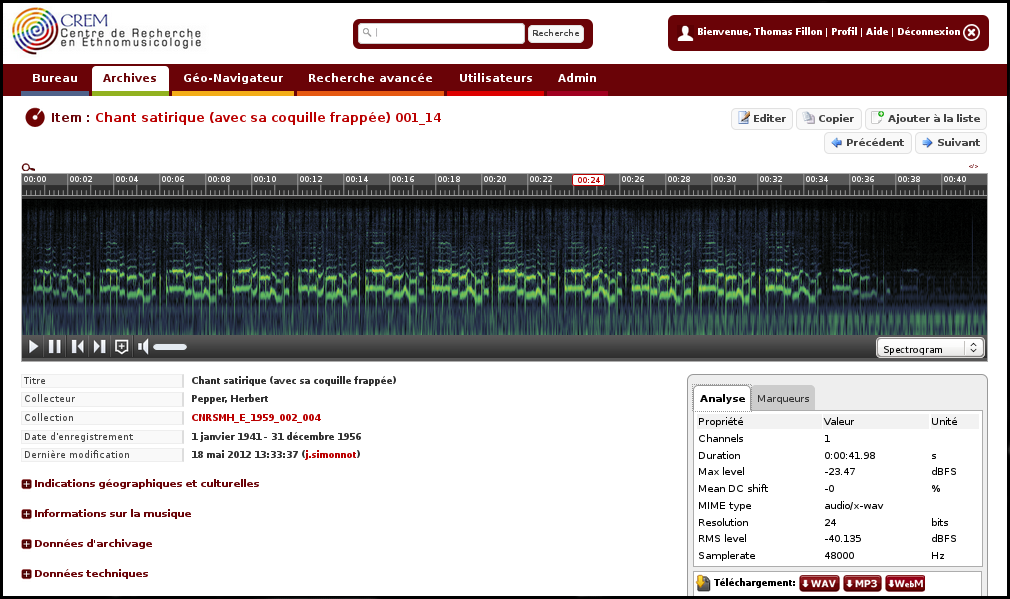
\includegraphics[width=0.4\paperwidth]{../img/telemeta.png}
  \caption{Screenshot excerpt of the \emph{Telemeta} web interface}\label{fig:Telemeta}
\end{figure}

\end{block}
\begin{block}{Metadata}\small
  \begin{itemize}
  \item In addition to the audio data, an efficient and dynamic
    management of the associated metadata is also required.
  \item Dynamically handling metadata in a collaborative manner optimises
    the continuous process of knowledge gathering and enrichment of
    the materials in the database.
  \item Compatibility : integration of the metadata standards protocols \emph{Dublin Core}
    and \emph{OAI-PMH} (Open Archives Initiative Protocol for Metadata
    Harvesting) \cite{DublinCore,OAI-PMH}.
  \end{itemize}

\textbf{Contextual Information}\\
In ethnomusicology, contextual information could be geographic, cultural and musical. It could also store archive related information and include related materials in any multimedia format. 

\textbf{Annotations and segmentation}\\
Metadata also consist in temporal information such as:
\begin{itemize}
\item a list of \emph{time-coded markers} associated with annotations
\item a list of of \emph{time-segments} associated with labels.
\end{itemize}
The ontology for those labels is relevant for ethnomusicology (e.g. speech versus singing voice segment, chorus, ...).
It should be noted that annotations and segmentation can be done either by a human expert or by some automatic signal processing analysis.

\end{block}
    \end{column}
   
% ==================================
% ------- Colonne droite -----------
% ==================================
\begin{column}[T]{.49\linewidth}
  \begin{block}{TimeSide}\small
One specificity of the Telemeta architecture is to rely on an external component, \emph{TimeSide}, that offers audio player integration together with audio signal processing analysis capabilities.
    \begin{figure}[htbp]
  \centering
  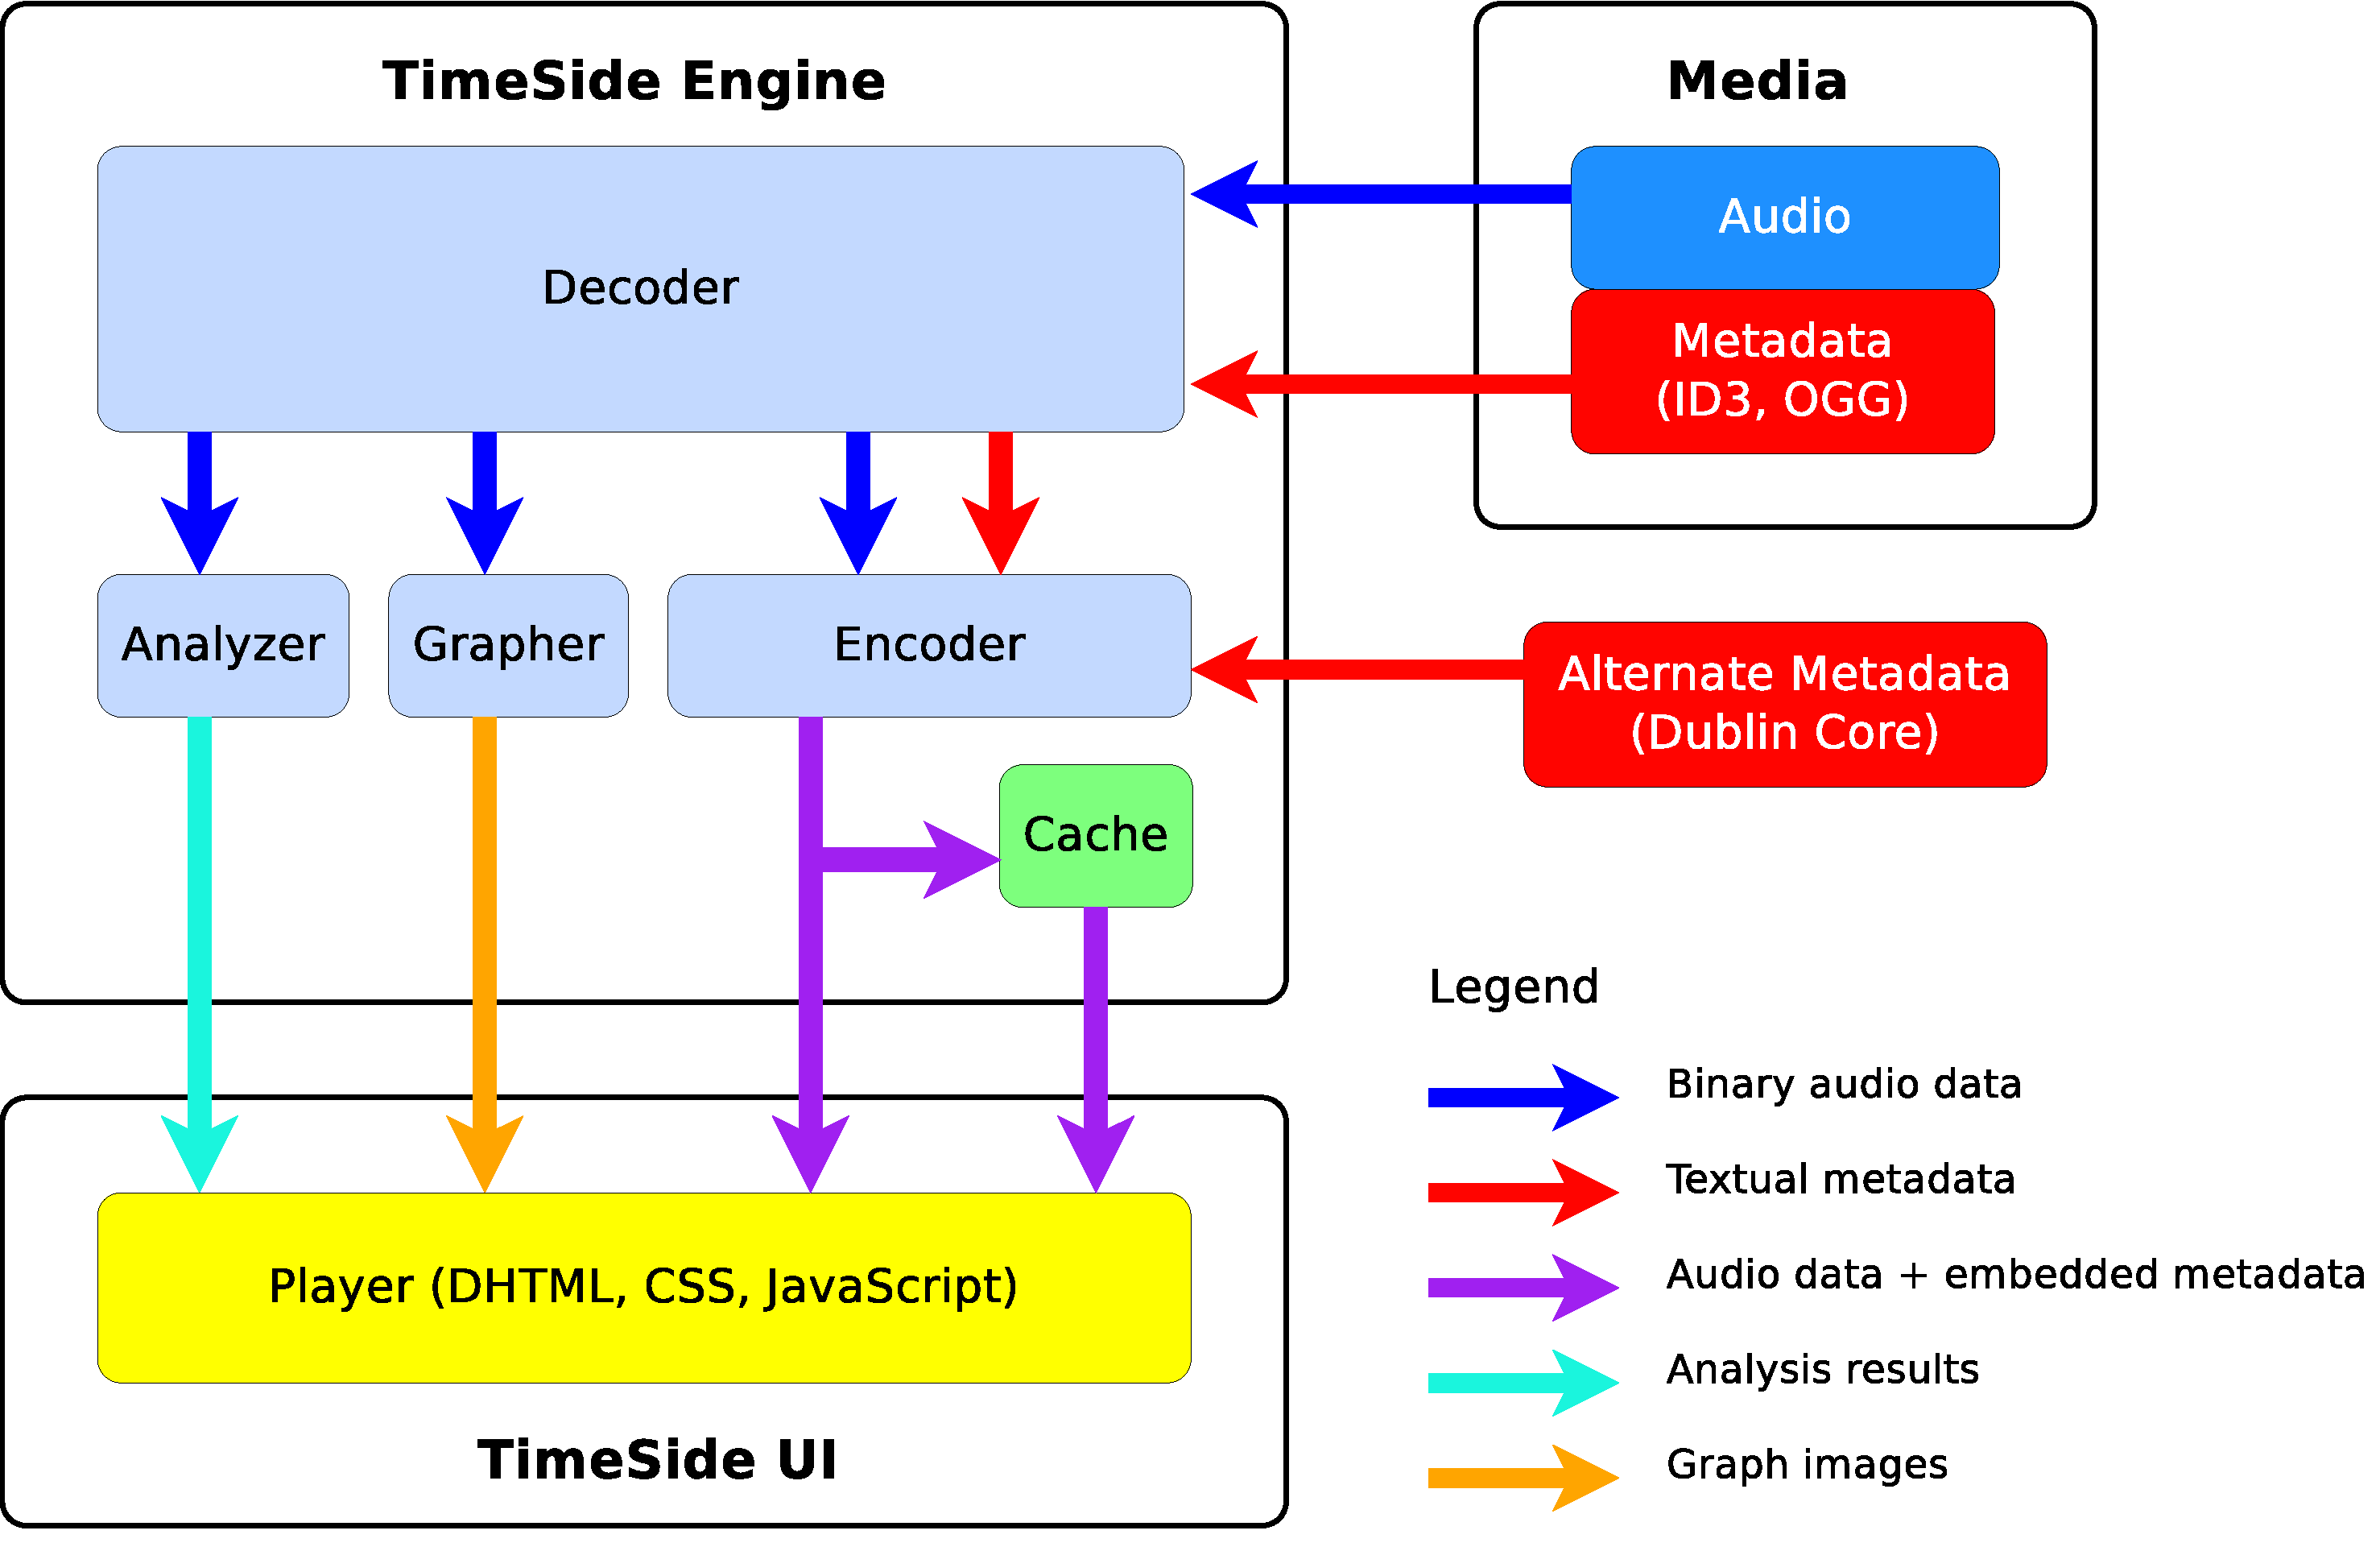
\includegraphics[width=0.4\paperwidth]{../img/timeside_schema.pdf}
  \caption{TimeSide architecture (see \url{https://code.google.com/p/timeside/})}\label{fig:TimeSide_Archi}
\end{figure}
\textbf{Audio management}\\
TimeSide provides the following main features:
\begin{itemize}
\item \emph{Secure archiving, editing and publishing of audio files} over
  internet.
\item Smart \emph{audio player} with enhanced visualisation (waveform, spectrogram)
\item \emph{Multi-format support}: reads all available audio and video formats  through Gstreamer, transcoding with smart streaming and caching methods
\item "On the fly" \emph{audio analyzing, transcoding and metadata
    embedding} based on an easy plugin architecture
\end{itemize}

\textbf{Audio features extraction}\\
TimeSide incorporates some state-of-the-art audio feature extraction libraries such as \href{http://aubio.org}{Aubio}, \href{http://yaafe.sourceforge.net}{Yaafe} and \href{http://www.vamp-plugins.org}{Vamp plugins} \cite{brossierPhD,yaafe_ISMIR2010,vamp-plugins}.
Given the extracted features, every sound item in a given collection can be automatically analyze. The results of this analysis can be displayed as a support to ethnomusicological studies.
Further works lead by the DIADEMS project will incorporate advance Music Information Retrieval methods in order to provide automatic annotation, segmentation and similarity analysis.
  \end{block}
  \begin{block}{Examples}\small
    
  \end{block}
\begin{block}{Références}\tiny
\bibliographystyle{../splncs03}
%\label{sec:ref}
\vspace{-1cm}
\begin{multicols}{2}[]
\bibliography{../cmmr_2013}
\end{multicols}
  \end{block}
 \end{column}
\end{columns}
\end{frame}
\end{document}
%%% Local Variables: 
%%% mode: latex
%%% TeX-master: t
%%% End: 
